\section{Overview of Explainable Artificial Intelligence}
\label{sec:xaiOverview}
eXplainable Artificial Intelligence (XAI) is not a new concept that has emerged recently. The earliest research on XAI can be traced back to literature published four decades ago \cite{explanation, explainingPrograms}, when certain expert systems were designed to provide explanations for their outputs based on the rules they applied. Scientists have been engaged in continuous discussions about the significance of explanations in intelligent systems, specifically concerning decision-making, since the beginning of AI research.

In the context of modern deep learning, however, XAI has emerged as a novel research area in response to the increasing complexity and opacity of machine learning models. It aims to provide insights into AI systems' decision-making processes and enable users to understand, trust, and effectively interact with these systems. The advent of XAI can be traced back to the early 2000s when Lipton raised a renewed interest in the field, emphasizing the importance of explainability in machine learning algorithms by his influence paper in 2016 \cite{startOfXAI}. Since then, the number of publications in the XAI domain has witnessed exponential growth, demonstrating the increasing attention and significance given to this area of research. For instance, a bibliometric analysis conducted by Park and Lehman revealed a staggering 350\% rise in the number of XAI-related papers published between 2017 and 2020 \cite{analysisOfXAI}.

The significant growth of XAI leads to a notable diversity of approaches and techniques. This diversity is a result of researchers' varying perspectives and goals in their pursuit of improving the interpretability of AI systems. Various taxonomies have been suggested in the research literature to categorize different explainability methods \cite{taxonomy, medicalXAI}. However, it is important to note that these classification techniques are not fixed or absolute. They can differ significantly based on the specific characteristics of the methods, and methods may fall into multiple classes that overlap or do not overlap. In this context, different types of taxonomies and classification approaches will be briefly discussed, while a more comprehensive analysis of these taxonomies can be found in the referenced source \cite{taxonomy}.
\begin{figure}
\centering
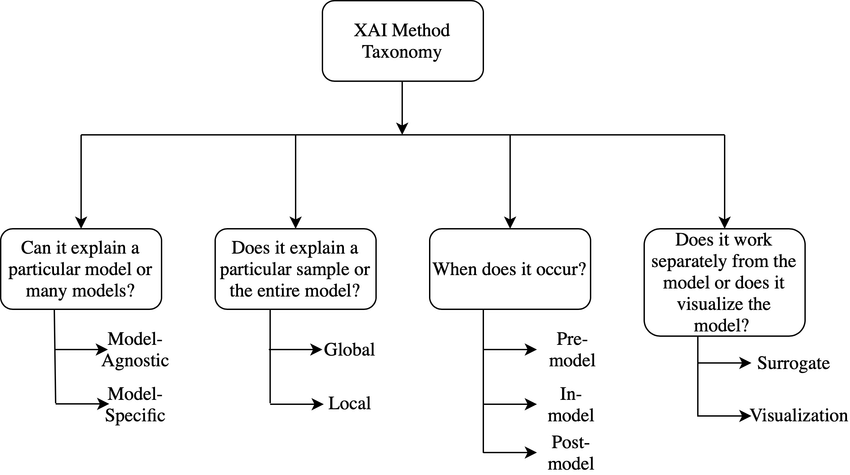
\includegraphics[width=13cm]{images/xai_methods/taxonomy-of-XAI-methods.png}
\caption{Taxonomy of XAI methods \cite{taxonomy}}
\end{figure}

One notable variation is the distinction between interpretable-by-design and post-hoc XAI methods. Interpretable-by-design XAI methods involve incorporating interpretability during the model's development phase. These methods focus on designing inherently interpretable models, such as decision trees or rule-based systems, which provide explicit rules for decision-making. By building models with transparency in mind from the outset, interpretable-by-design methods offer direct interpretability without the need for additional post-hoc explanations. On the other hand, post-hoc XAI methods are applied after the model has been trained and are commonly used with black-box or complex models, including deep neural networks. These methods seek to explain the model's predictions without modifying its internal workings. Post-hoc XAI methods provide an additional layer of interpretability by generating explanations that are independent of the underlying model's architecture or learning algorithm.

Post-hoc XAI methods can be further categorized based on their approaches. A model-specific method is tailored to a particular machine learning model or architecture, leveraging its internal structure and characteristic to generate explanations. These methods include techniques like Layer-wise Relevance Propagation (LRP) \cite{lrp}, which rely on understanding the inner workings of deep neural networks. On the other hand, model-agnostic approaches, such as Local Interpretable Model-Agnostic Explanations (LIME) \cite{lime} and Shapley Additive Explanations (SHAP) \cite{shap}, aim to provide explanations that are independent of the underlying model. These methods generate explanations by approximating the model's behavior through sampling or perturbing the input data.

Another aspect of variation in XAI methods is the granularity of explanations. Some techniques focus on generating global explanations, providing insights into the overall behavior of the model across the entire dataset or feature space. Integrated Gradients \cite{IG} is an example of techniques that offer global explanations by assessing the impact of different features on model predictions. In contrast, local explanation methods concentrate on explaining individual predictions or instances. These methods, such as LIME \cite{lime} and SHAP \cite{shap}, highlight the specific features that influenced a particular prediction, providing more fine-grained explanations.

XAI methods also vary in terms of the types of explanations they generate. Some methods utilize textual or rule-based explanations to provide human-readable justifications for model decisions. Rule extraction techniques, for instance, aim to extract understandable rules from complex models, enabling users to comprehend the decision-making process. Other methods employ visualizations, such as saliency maps, to visually highlight important regions or features in the input data that contribute to model predictions. In this work, we will focus on this difference between explanations via saliency maps. 

\section{Overview of Saliency-based XAI Methods}
\label{sec:saliencyMapOverview}
The concept of saliency maps \cite{saliencyMaps} is based on the idea that certain regions or pixels in an image or input data play a crucial role in the model's prediction. By assigning importance scores to each pixel, saliency maps highlight the areas that have the highest influence on the model's output. This section outlines various saliency map explanation methods/algorithms that will be employed in our thesis. The methods can be categorized into two groups, depending on the approach they utilize to calculate the contribution of each input pixel value: Gradient-based and Perturbation-based.
 
\subsection{Gradient-based methods}
\label{subsec: gradientMethods}
%Dựa trên giả định rằng ta có khả năng biết được các tham số của các mô hình dự đoán, các phương pháp dựa trên đạo hàm trước tiên suy luận nhãn lớp bằng quá trình forward pass và sau đó sử dụng nhãn đã dự đoán để truyền ngược qua từng lớp trong mô hình dự đoán theo thứ tự đến tầng đầu vào để ước tính các đóng góp của đầu vào trong quá trình back propagation. Các phương pháp này dựa trên đạo hàm tạo ra saliency map cho thấy đóng góp của mỗi biến số trong không gian đầu vào đến dự đoán cuối cùng của mạng \cite{gradientBased}. Một lợi thế nữa của các phương pháp gradient-based là một (hoặc một vài) lần forward pass và back propagation giúp ta đánh giá được độ đóng góp của tất cả các đặc trưng trong đầu vào (global contribution).

Based on the assumption that we know the parameters in the black box model, gradient-based methods first produce predictions through a forward pass and then utilize the predicted labels to propagate backward through each layer of the model, in sequential order, all the way to the input layer, estimating the contributions of the inputs during the backpropagation process. These methods, relying on derivatives, generate saliency maps that illustrate the contributions of each variable in the input space to the final prediction of the black box \cite{gradientBased}. Another advantage of gradient-based methods is that a single (or a few) forward pass and backpropagation allow us to evaluate the contributions of all features in the input (global contribution).

\subsubsection{Vanilla Gradient/Saliency}
\label{subsubsec: grad}
Saliency method \cite{saliencyMaps} was one of the initial approaches developed to visualize the input attribution of convolutional networks. As the term ``saliency'' is commonly associated with the overall approach of displaying input attribution known as the Saliency maps, this particular method is also referred to as Vanilla Gradient.
The concept of the Saliency method originates from class visualization, which involves finding an image $I$ that maximizes the score $S_c$ for a particular class $c$ while incorporating $L2$ regularization. Formally, this can be expressed as follows:
\begin{equation}
    \underset{I}{argmax}(S_c (I) - \lambda \norm{I} ^2_2)
\end{equation}

In the case of deep CNN models, the class score $S_c(I)$ is a highly non-linear function. However, we can approximate the class score $S_c(I)$ with a linear function in the neighbourhood of an image $I_0$ by utilizing the first-order Taylor expansion.
\begin{equation}
    S_c(I) \approx w^T I + b
\end{equation}

To compute the saliency map $A$, we just arrange the values in $w$ to match the shape of input image $I$ 
\begin{equation}
A_{i, j} = \underset{ch}{max}\abs{w_{h(i, j, ch)}}
\end{equation}
 where $ch$ is a color channel of the pixel $(i,j)$ and $h(i,j,ch)$ is an index of the $w$ corresponding to the same pixel $(i,j)$ and $w$ is the derivative of $S_c$ with respect to the image I at the image $I_0$

\begin{equation}
    w = \frac{\partial S_c}{\partial I} \bigg \rvert_{I_0}
\end{equation}

\subsubsection{Integrated Gradient}
\label{subsubsec: IG}
Integrated Gradients (IG) is an approach proposed by Sundararajan et al. \cite{IG} in 2017. This method is based on two axioms to which the authors assert that these principles should be upheld by all attribution methods: Sensitivity and Implementation Invariance. The specific definition of those two axioms is as follows:

\begin{itemize}
    \item Sensitivity:
An attribution method satisfies Sensitivity when it meets two conditions:
The first condition is if we have two inputs and baselines that differ in only one feature, but result in different predictions by the model, then the feature that distinguishes them should be assigned a non-zero attribution. In other words, when a single feature alteration leads to divergent model outputs, the attribution method should correctly identify and highlight the contribution of that differing feature.

The second condition is if the function implemented by the model does not depend (mathematically) on a particular variable or feature, then the attribution assigned to that variable should always be zero. In other words, if a feature has no influence on the model's predictions or decision-making process, it should not be attributed any significance or contribution.
    
    \item Implementation Invariance: The attribution values must be the same if two models are equivalent - Two models are considered functionally equivalent if their outputs are the same for all possible inputs, even if they have been implemented using different architectures or methodologies. The goal of Implementation Invariance is to ensure that the attributions produced by an attribution method remain consistent and identical when applied to functionally equivalent networks.
\end{itemize}

%Kỹ thuật Integrated Gradient tính độ biến thiên kết quả đầu ra của mô hình giữa đầu vào $x$ và tham chiếu $x'$ (trên mô hình với tác vụ hình ảnh, baseline $x'$ có thể là ảnh với tập các pixel giá trị 0 - ảnh đen) bằng cách tính tích phân đường độ biến thiên của đầu ra trên vector $x' \rightarrow x$. Cụ thể, giả sử mô hình của chúng ta được biểu diễn dưới dạng toán học là một hàm số $F: R^n \rightarrow [0, 1]$, công thức tính độ biến thiên đầu ra trên từng biến đầu vào  $\frac{F(x_i)}{x_i}$ như sau: 
The main idea of this technique is to quantify the change in model output between an input $x$ and a reference baseline $x'$ (in the case of an image task, the baseline $x'$ is often represented as a black image with all pixels set to 0). To compute the output variation, IG calculates the gradient of the model's output with respect to the input variables along the path from $x'$ to $x$. The main idea is to integrate the gradients over this path to obtain a comprehensive measure of the input variable's impact on the model's output.

Let's assume our model is a mathematical function denoted as $F: R^n \rightarrow [0, 1]$, where $n$ represents the number of input variables. The formula used to calculate the output variation attributed to each input variable, $x_i$, is as follows:

\begin{equation} \label{ig_formula}
IG_i(x_i) = (x_i - x'_i) \times \int_{\alpha = 0}^{1} \frac{\partial F(x'_i + \alpha \times (x_i - x'_i))}{\partial x_i}d\alpha 
\end{equation}
By evaluating this integral for each input variable, this technique quantifies the contribution of each variable to the model's output variation between the input and the baseline. This provides valuable insights into the relative importance and influence of different input features on the model's decision-making process.

\subsubsection{Grad-CAM}
\label{subsubsec:GC}
%Grad-CAM (Gradient-weighted Class Activation Mapping) \cite{grad_cam} là một phiên bản tổng quát hơn của CAM (class activation mapping) \cite{cam_zhou}. Với phương pháp CAM, kiến trúc của các mô hình cần áp dụng phép toán Global Average Pooling (GAP) ở lớp tích chập (convolutional) cuối cùng và một lớp fully-connected ở cuối để mô hình đưa ra dự đoán. Với kiến trúc này, để giải thích, ta sẽ dùng kết quả có được sau khi thực hiện phép toán GAP trên các feature map activations, đánh trọng số chúng dựa trên trọng số của lớp phân loại cuối cùng để tạo ra class activation map. Cụ thể, gọi $F_k = \sum_{x, y} {f_k(x,y)}$ là kết quả của phép GAP lên feature map activation k tại điểm $(x, y)$, class activation map của phân lớp $c$ - $M_c$ được tính như sau:

Grad-CAM (Gradient-weighted Class Activation Mapping) \cite{grad_cam} is a more general version of CAM (Class Activation Mapping) \cite{cam_zhou}. With CAM, the model architecture requires the use of Global Average Pooling (GAP) operation at the last convolutional layer followed by a fully-connected layer to make predictions. With this architecture, to explain the model's decision, we utilize the results obtained after performing GAP on the feature map activations and weight them based on the weights of the final classification layer to generate a class activation map. Specifically, let $F_k = \sum_{x, y} {f_k(x,y)}$ represent the result of applying GAP to the activation feature map $k$ at the point $(x, y)$. The class activation map for class $c$, denoted as $M_c$, is calculated as follows:

\begin{equation}
M_c(x, y) = \sum_{k} F_k w_k^c
\end{equation}

In this equation, $w_k^c$ represents the weight associated with the $k$-th activation feature map for the class $c$. By summing up the weighted feature map activations, the Grad-CAM technique generates a class activation map that attributes the regions of the input image that contribute most significantly to the prediction for the target class.

By visualizing the class activation map, we can identify the spatial locations within the input image that the model focuses on when making predictions. These regions often correspond to the discriminative features relevant to the target class, providing insights into the model's decision-making process.

%Ý tưởng của Grad-CAM vẫn là sử dụng những feature maps có được từ lớp tích chập mà ta chọn  để tính giá trị đóng góp từ đầu vào. Điểm khác biệt là ta đánh trọng số feature maps bằng giá trị $\alpha$ được tính theo gradient. Cụ thể, thuật toán Grad-CAM gồm 3 bước sau:
Grad-CAM generalizes the CAM approach by eliminating the requirement of the model architecture. It leverages the gradient information flowing into the convolutional layers. This makes Grad-CAM applicable to a wide range of CNN architectures. The idea behind Grad-CAM remains using feature maps obtained from the chosen convolutional layer to calculate the contribution values from the input. The difference lies in weighting the feature maps using the gradient-derived value, denoted as $\alpha$. Specifically, the Grad-CAM algorithm consists of the following three steps:

Step 1: Calculate the variation of the output value for class $c$, denoted as $y_c$, with respect to the activation feature map $A^k$ in the desired convolutional layer that we want to explain.

Step 2: Compute the weight $\alpha$ for the $k$-th activation feature map using the formula:
\begin{equation}
\alpha_k^c = \frac{1}{Z} \sum_i \sum_j \frac{\partial y^c}{\partial A^k_{ij}}
\end{equation}
%
Here, $\frac{\partial y^c}{\partial A^k_{ij}}$ represents the partial derivative of the output class $c$ with respect to the activation feature map $A^k_{ij}$ at position $(i, j)$, and $\frac{1}{Z}\sum_i \sum_j$ works as Global Average Pooling

Step 3: After obtaining the weights $\alpha$, we can calculate the Grad-CAM heatmap by summing the weighted feature map activations and applying the ReLU function. Specifically, the Grad-CAM heatmap for class $c$ is computed as follows:
\begin{equation}
L^c = \text{ReLU}\left(\sum_k{\alpha_k^c A^k}\right)
\end{equation}
%
The ReLU function is used here to consider only positive contribution values, while negative values are set to 0.

By following these steps, Grad-CAM generates a heatmap that highlights the important regions of the input image for the predicted class. These regions correspond to the areas where the model focuses its attention when making predictions. The higher the intensity in the Grad-CAM heatmap, the more influential the corresponding spatial locations are in determining the prediction for the target class.

\subsubsection{Guided Backpropagation}
\label{subsubsec:GBP}
%Guided Backpropagation \cite{guidedbackprop} (GBP) là một phương pháp giải thích dựa trên cơ chế lan truyền ngược (backpropagation). Ý tưởng của GBP được Alexey Dosovitskiy và đồng nghiệp phát triển dựa trên Deconvolution \cite{deconv} và Saliency \cite{saliencyMaps}. Tác giả nhận định rằng phương pháp Saliency \cite{saliencyMaps} của Simonyan có vấn đề nếu có sự tham gia của các gradient giá trị âm, thứ làm giảm độ chính xác của các lớp sâu trong mô hình mà ta đang cố giải thích. Để giải quyết, tác giả đã kết hợp 2 phương pháp lại, thêm chỉ dẫn vào phương pháp Saliency với sự giúp đỡ của Deconvolution
%Kỹ thuật này kèm theo từ "guided" vì cho phép chúng ta chọn những neuron nào được kích hoạt để thực hiện quá trình backpropagation. Để làm việc đó, phương pháp này chỉnh sửa bước backpropagation thông thường bằng phép tính ReLU để chỉ backpropagation những giá trị gradient dương. Các giá trị gradient âm sẽ được gán bằng 0. Cụ thể, gọi $f^l_i$ là feature map ở layer thứ $l$, kết quả lan truyền ngược ở layer $l$ được tính như sau:

Guided Backpropagation (GBP) \cite{guidedbackprop} is an explanation method based on the backpropagation mechanism. The idea behind GBP was developed by Alexey Dosovitskiy et al. building upon Deconvolution \cite{deconv} and Saliency \cite{saliencyMaps} techniques. The authors argued an issue with the Saliency method proposed by Simonyan \cite{saliencyMaps}, which arises when negative gradient values are involved. These negative gradients could decrease the accuracy of deeper layers in the network being explained. To address this issue, the authors combined the two methods and introduced guidance into the Saliency method with the help of Deconvolution.

The term ``guided'' in this technique implies that we can selectively activate specific neurons to perform the backpropagation process. To achieve this, the method modifies the standard backpropagation step using the ReLU operation, allowing only positive gradients to be backpropagated. Negative gradient values are assigned a value of 0. Specifically, let $f^l_i$ denote the feature map at layer $l$, and the backpropagation result at layer $l$ is computed as follows:

\begin{equation}
\frac{\partial E}{\partial f^l_i} = \max\left(0, \frac{\partial E}{\partial f^{l+1}_i}\right) \cdot \frac{\partial f^{l+1}_i}{\partial f^l_i}
\end{equation}
%
Here, $\frac{\partial E}{\partial f^l_i}$ represents the backpropagated error with respect to the feature map $f^l_i$ at layer $l$. The ReLU operation ensures that only positive gradients are considered, filtering out negative gradients during the backpropagation process.

Guided Backpropagation is particularly useful when we want to focus on specific neurons or regions of the model during the explanation process. By selectively activating certain neurons and propagating positive gradients, GBP allows us to highlight the influential features and understand the model's decision-making process at a more fine-grained level.

\subsubsection{Guided GradCAM}
\label{subsubsec: GGCAM}
%Guided Grad-CAM kế thừa thứ mà Grad-CAM \ref{subsubsec:GC} làm tốt nhất là phân lớp (class-discrimation) và định vị (localization) với khả năng trực quan hoá bằng cách chỉ tính đóng góp ở những nơi gradient dương của phương pháp Guided Backpropagation \ref{subsubsec:GBP}
Guided GradCAM is an XAI method that combines the principles of Grad-CAM \ref{subsubsec:GC} and Guided Backpropagation to provide more localized and fine-grained explanations of deep neural network predictions. Guided Grad-CAM inherits the strengths of Grad-CAM, which are class discrimination and localization, with the ability to visualize by focusing only on the contributions in regions with positive gradients from the Guided Backpropagation method.

The main idea behind GuidedGradCAM is to generate a heatmap that represents the importance of each pixel or region in the input with respect to the predicted class. This heatmap is obtained by combining the gradient information from both the Grad-CAM and Guided Backpropagation methods. To combine these two methods, GuidedGradCAM utilizes the positive gradients obtained from Guided Backpropagation and multiplies them element-wise with the Grad-CAM weights. This multiplication enhances the relevance of positive features while suppressing the influence of negative features. The resulting guided Grad-CAM heatmap provides a more focused and accurate representation of the important regions in the input.
Mathematically, let's denote the Grad-CAM weights for class $c$ as $W_c$ and the guided backpropagated gradients as $L_{\text{guided}}$. The GuidedGradCAM heatmap $H_c$ for class $c$ is obtained by element-wise multiplication of these two quantities:
\begin{equation}
H_c = \text{ReLU}(W_c \odot L_{\text{guided}})
\end{equation}
where $\odot$ represents element-wise multiplication and ReLU ensures that only positive contributions are considered.

\begin{figure}[ht]
\centering
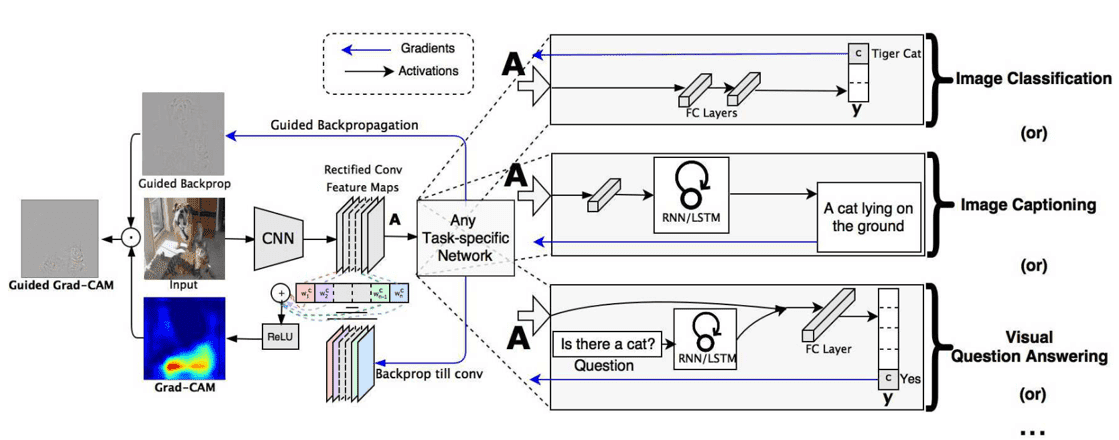
\includegraphics[width=13cm]{images/xai_methods/guided-grad-cam.png}
\caption{How Guided Grad-CAM heatmaps generated by combining Grad-CAM \& Guided backpropagation method. Source \cite{grad_cam}}
\end{figure}

The resulting heatmap $H_c$ highlights the regions in the input that have a strong positive influence on the prediction for class $c$. These regions indicate the areas that the model focuses on when making the prediction and provide insights into the important visual cues or features.

\subsubsection{Layer-wise Relevance Propagation}
\label{subsubsec:lrp}
Layer-wise Relevance Propagation (LRP) was introduced by Bach et al. \cite{lrp}. The fundamental idea behind LRP is to assign relevance scores to the input features or neurons based on their impact on the model predictions. LRP achieves this by redistributing the output relevance backward through the layers of the neural network.

LRP adheres to the conservation property, which states that the relevance received by a neuron must be evenly redistributed to the neurons in the lower layer. In simpler terms, whatever relevance a neuron receives, it must pass on an equal amount of relevance to the neurons in the next layer. This conservation property is one of the fundamental principles of LRP, although there are other properties that LRP also follows, this particular property is explicitly emphasized in its implementation. Let's denote $j, k$ are two consecutive layers, $z_{jk}$ quantifies the amount of contribution node $j$ has to make node $k$ relevant, $z_{jk} = x_j^{(l)}w_{jk}^{(l, l+1)}$, the guiding equation for propagating relevance scores is:

\begin{equation}
\label{equation:conservation}
    R_j = \sum_{k}{\frac{z_{jk}}{\sum_j{z_{jk}}}}R_k
\end{equation}

\begin{figure}[hbt!]
\centering
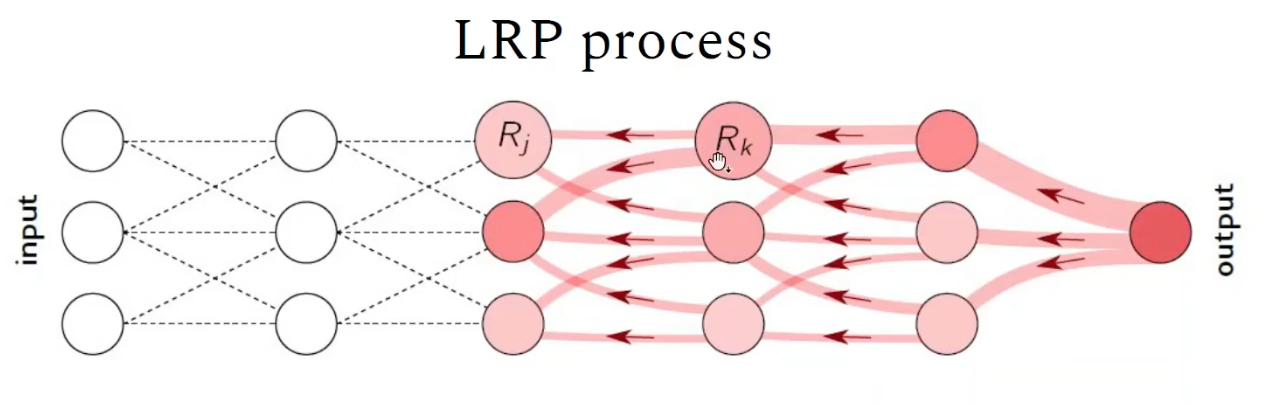
\includegraphics[width=13cm]{images/xai_methods/lrp.png}
\caption{Relevance scores propagating procedure. Source \cite{lrp}}
\end{figure}

This relevance redistribution is guided by certain rules and principles that ensure the preservation of relevance throughout the network. One commonly used rule in LRP is the ``epsilon rule'' which solves the problem of gradient noise by introducing a small positive term, $\epsilon$ to the denominator

The $\epsilon$-rule formula for LRP can be expressed as follows:
\begin{equation}
    R_j = \sum_{k}{\frac{z_jk}{\epsilon + \sum_i{z_{jk}}}}R_k
\end{equation}

An advantage of LRP is the consideration of both positive and negative contributions. This helps in understanding not only the positive factors that drive the model's prediction but also the inhibitory factors that may counteract certain features or neurons.

LRP is a broad family of methods, and different variants and modifications exist to adapt to various network architectures and specific application domains. The choice of propagation rules and modifications may vary depending on the specific requirements and interpretability objectives.

\subsubsection{Deep Label-Specific Feature Learning}
\label{subsubsec:deeplift}
While LRP adhered to the conservation axiom, which ensures that the relevance received by a neuron is redistributed equally to the lower layer, there was still a challenge in determining how to allocate the net relevance among individual pixels within a layer. This ambiguity led to difficulties in accurately understanding the contribution of each pixel to the overall relevance. To address this issue, Deep Label-Specific Feature Learning (DeepLIFT) \cite{deeplift} introduces an additional axiom on how to propagate the relevance down. 

DeepLIFT calculates the contributions of individual neurons by comparing their current activation with a reference activation. The reference activations for all neurons are determined by performing a forward pass, where the input parameters are propagated through the neural network. More details are presented in \cite{deeplift}. In simple terms, to explain a neural $x$, let's denote $t$ as its current activations and $t'$ as its reference activation. If the difference between these two values $\delta t = t - t'$, DeepLIFT assigns contribution scores $C_{\delta x_i \delta t}$ to $\delta x_i$ as follows:

\begin{equation}
\label{equation:deeplift}
    \sum_{i = 1}^{n} C_{\delta x_i \delta t} = \delta t
\end{equation}

\subsubsection{Gradient SHapley Additive exPlanation}
\label{subsubsec:gradshap}

GradientSHAP (Gradient SHapley Additive exPlanation) \cite{shap} combines the gradient-based approach to attribution and  the concepts of Shapley values from cooperative game theory.

In cooperative game theory, Shapley values are used to fairly distribute the contribution among players in a cooperative game. In the context of XAI, Shapley values measure the contribution of each feature to the prediction or output of the model.

To calculate the Shapley value of a feature, we consider all possible permutations of the features and measure their marginal contributions. In each permutation, we determine the difference in the prediction when the feature is included versus when it is not. By averaging these differences across all permutations, we obtain the Shapley value for that feature. Suppose $F$ is the set of all features, S is all feature subsets of $F$. We compute the contribution value of a feature $i$ as in the formula \ref{equation:shap} represented in the work of Scott et al. \cite{shap}.

\begin{equation}
\label{equation:shap}
\phi_i = \sum_{S \subset F \cup \{i\}} \frac{\abs{S}!(\abs{F} - \abs{S} - 1)!}{\abs{F}! } ( f_{S \cup \{ i \}} ( x_{ S \cup \{ i \}} ) - f_S (x_S) )
\end{equation}
where $f_K$ is a model trained with the set of feature $K$.

With GradientSHAP, the Shapley values are computed using gradients. Gradients provide information about how changes in feature values affect the model's output. By considering the gradients of the model's predictions with respect to the input features, GradientSHAP determines the relative importance of each feature in the prediction process. Here's an overview of how the GradSHAP works:
 
1. Choose a reference dataset: Select a dataset that represents the background or baseline data distribution. This dataset serves as a reference point for calculating SHAP values.
 
2. Compute the expected model output: Calculate the average prediction of the model across the reference dataset. This provides the expected value of the model output, denoted as $E[f(x)]$.
 
3. Calculate the gradients: Determine the gradients of the model output with respect to the input features for a specific instance. Gradients indicate the rate of change of the model output for each feature. $\nabla_x f(x)$.
 
4. Combine the gradients with the expected values: To approximate the SHAP values, we linearize the model output around the expected values using the computed gradients. Therefore, the approximation of the SHAP value for each feature can be calculated as:
$$\phi_i = \sum_{j=1}^N (x_j - E[x_j]) \cdot \nabla_{x_j} f(x)$$
where $\phi_i$ is the SHAP value for the $i$-th feature, $N$ is the number of features, $x_j$ is the value of the $j$-th feature for the input instance $x$, and $E[x_j]$ is the expected value of the $j^{th}$ feature calculated from the reference dataset.
 
5. Calculate the SHAP values: The above formula gives an approximation of the SHAP values for each feature. To improve the accuracy, we can use different reference instances for each feature and average the results. This can be done by sampling multiple times from the reference dataset and computing the SHAP values for each sample, then averaging the results. This process is called Monte Carlo sampling.

In summary, the SHAP Gradient Explainer uses the gradients of the model output with respect to input features to approximate SHAP values, which provide a fair distribution of the contribution of each feature towards the prediction for a specific instance.
\subsection{Perturbation-based methods}
\label{subsec:perturbationMethods}
% Khác với các phương pháp gradient-based, những phương pháp perturbation-based phân tích cách các kết quả dự đoán của mô hình thay đổi khi một hoặc nhiều đặc trưng đầu vào bị biến đổi, điều này khiến cho các phương pháp này trở thành lựa chọn tối ưu cho việc phân tích độ nhạy cảm (sensitivity) của các mô hình \cite{gradientBased}. Phân tích độ nhạy cảm của các mô hình trở nên đặc biệt quan trọng khi ta phải đối mặt với những cuộc tấn công mà ở đó những thay đổi ở đầu vào được thiết kế một cách cẩn thận nhằm mục đích cố ý thay đổi kết quả đầu ra của mô hình - "adversarial attack" \cite{adversarialAttacks}. Các phương pháp perturbation-based chỉ cần thực hiện một hoặc nhiều lần chuyển tiếp nhưng lại tốn rất nhiều chi phí tính toán so với các phương pháp gradient-based do phải thực nghiệm trên tập gồm càng nhiều biến động được tạo ra càng tốt. Ngoài ra, kết quả đầu ra của các phương pháp này không mang tính tổng quát mà chỉ chính xác với tập những biến động mà chúng ta tạo ra khi thử nghiệm.
Unlike gradient-based methods, perturbation-based methods analyze how the model's predictions change when one or more input features are perturbed. These perturbations can be in the form of adding noise, modifying pixel values, or altering specific features in a controlled manner. By observing how the model's predictions change in response to these perturbations, we can gain insights into the importance and impact of different features on the model's decision-making process.

The process of perturbation-based analysis typically involves generating multiple perturbed versions of the input and evaluating the model's predictions for each perturbed instance. This analysis provides a more comprehensive understanding of how variations in input features influence the model's output. This characteristic makes perturbation-based methods an optimal choice for analyzing the sensitivity of models \cite{gradientBased}. Analyzing the sensitivity of models becomes particularly important when dealing with attacks where carefully crafted input modifications intentionally aim to alter the model's output, known as ``adversarial attack'' \cite{adversarialAttacks}.  

However, perturbation-based methods come with computational costs due to the need for generating and evaluating a large number of perturbed samples. The generated perturbations should ideally cover a diverse range of possible variations to ensure a robust analysis. Furthermore, perturbation-based methods require multiple forward passes which are computationally expensive compared to gradient-based methods since they need to experiment with a diverse set of generated perturbations. This computational burden limits the scalability and efficiency of perturbation-based methods, especially when dealing with complex models and high-dimensional input spaces.

It is worth noting that the results obtained from perturbation-based methods are specific to the generated sample and may not capture the model's behavior under all possible samples in input space. Therefore, the interpretability provided by perturbation-based methods is constrained to the tested perturbations and may not fully represent the model's general behavior.

\subsubsection{Occlusion}
\label{subsubsec:occlusion}
%Occlusion là một phương pháp giải thích đánh giá đóng góp của từng vùng cụ thể trong ảnh bằng cách che phủ hoặc làm mờ các vùng quan tâm trong ảnh và theo dõi sự thay đổi trong kết quả đầu ra của mô hình. Gọi giá trị đầu vào ban đầu là $x$, mô hình được thể hiện dưới dạng hàm số $f: \in R^m \rightarrow R^n$ . Một vùng trong ảnh được chọn để occlusion để che phủ, với ảnh đã được che mất một vùng ảnh là $x_occ$, độ đóng góp của vùng ảnh đó  được tính như sau:
The main idea behind the Occlusion technique is to systematically occlude different regions of the input data and observe the resulting changes in the model's predictions \cite{deconv}. By comparing the predictions before and after occlusion, we can infer the importance or relevance of the occluded regions in influencing the model's decision.

To apply the Occlusion method, we slide a predefined occlusion window across the input data, systematically covering different regions. The occlusion window can have various shapes and sizes depending on the nature of the input data. At each occlusion position, we replace the occluded region with a neutral value (e.g., zero or average value) and feed the modified input to the model to obtain a new prediction.

The difference between the original prediction and the prediction with the occlusion indicates the importance of the occluded region. Larger deviations in predictions suggest that the occluded region played a more influential role in the model's decision-making process.

Mathematically, let's denote the original input as $x$ and the occluded input as $\tilde{x}$ obtained by occluding a specific region. The model's prediction on the original input is $f(x)$, and the prediction on the occluded input is $f(\tilde{x})$. The occlusion score, representing the importance of the occluded region, can be calculated using a similarity measure, such as the difference in predictions:
\begin{equation}
\text{Occlusion Score} = f(x) - f(\tilde{x})
\end{equation}

The advantage of Occlusion is that it does not rely on gradient information and can be applied to various types of models, including non-differentiable models. However, its effectiveness depends on the choice of the occlusion window size, shape, and stride, as well as the definition of the neutral value used for occlusion. Additionally, occluding small, local regions may not capture the global interactions between features in the input, potentially leading to limited interpretability.